\hypertarget{a00008}{
\section{Dokumentacja pliku debug.hpp}
\label{d4/dee/a00008}\index{debug.hpp@{debug.hpp}}
}
{\tt \#include $<$cstdio$>$}\par
{\tt \#include $<$cstdlib$>$}\par


Wykres zależności załączania dla debug.hpp:\nopagebreak
\begin{figure}[H]
\begin{center}
\leavevmode
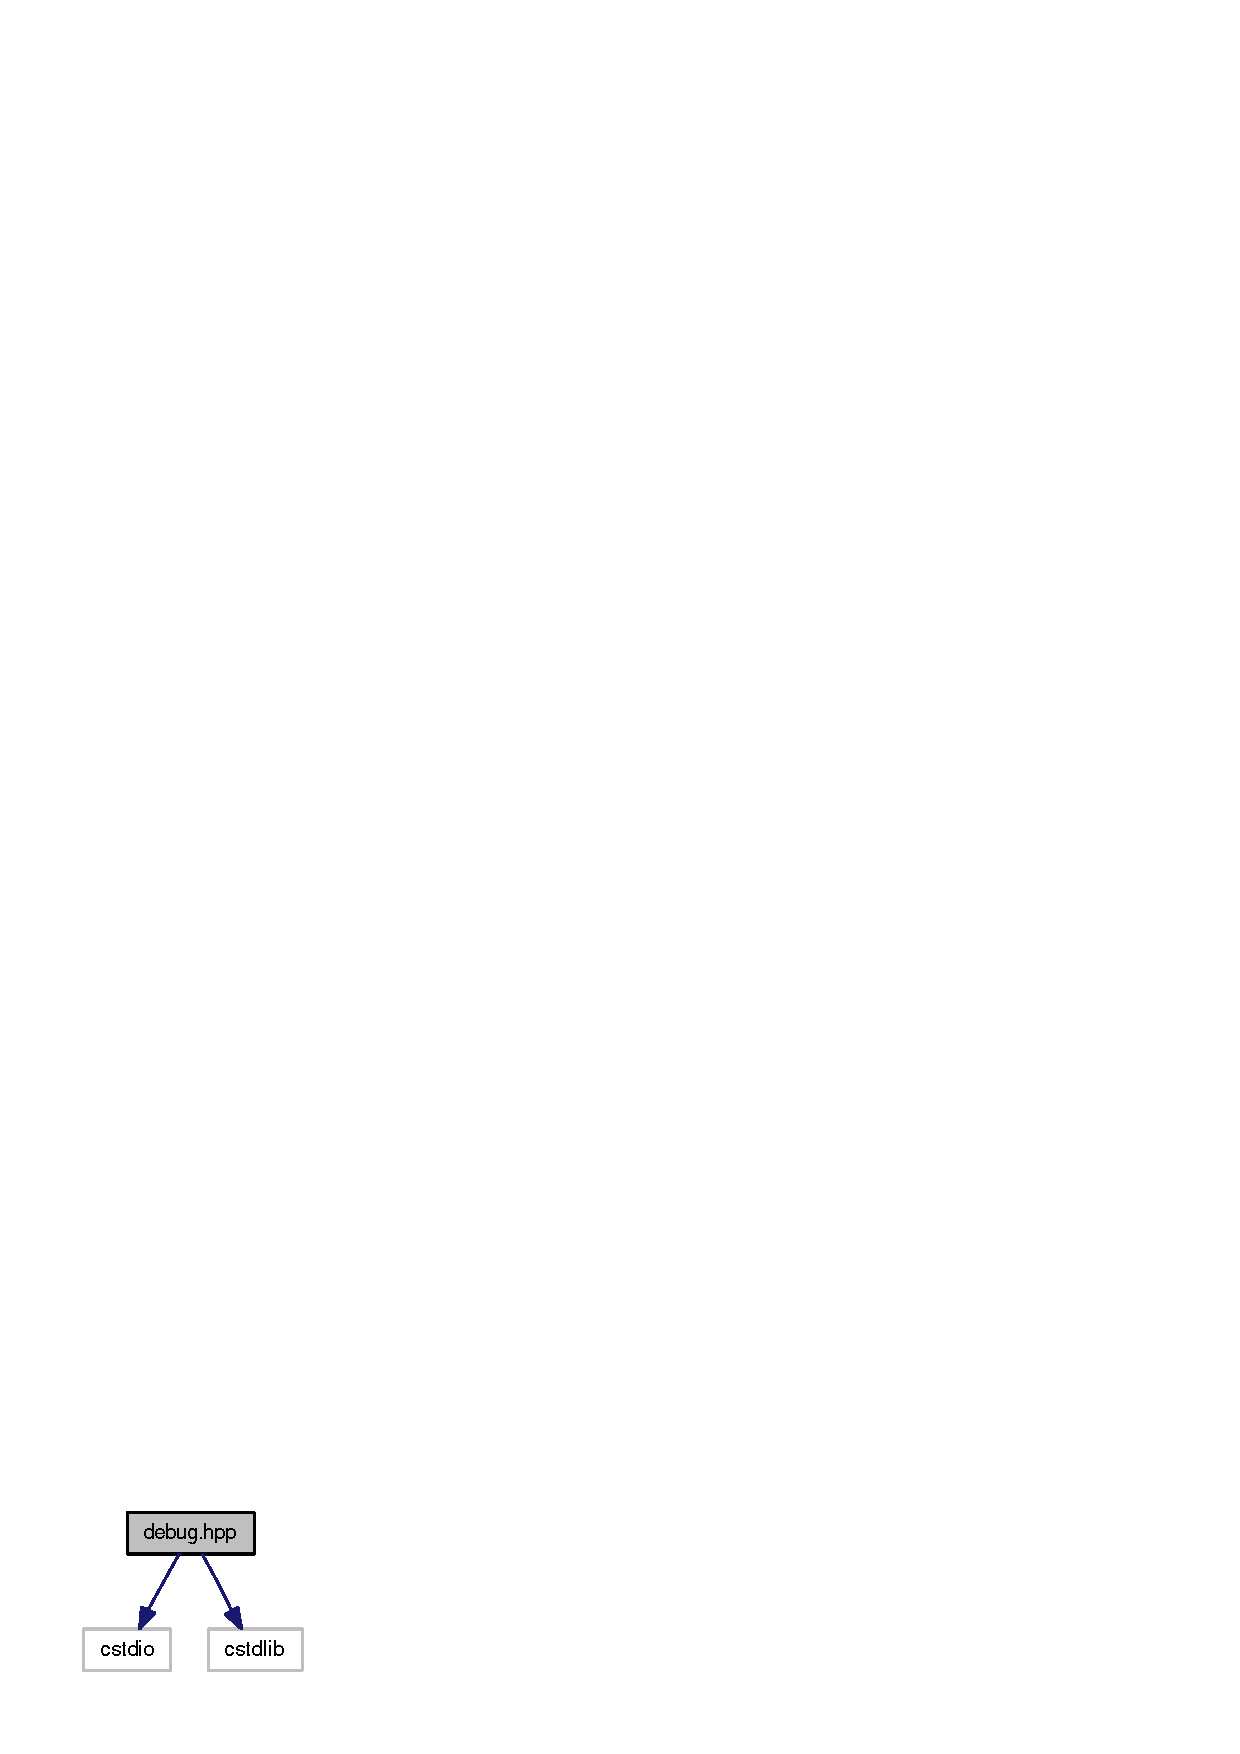
\includegraphics[width=74pt]{d1/dc6/a00037}
\end{center}
\end{figure}


Ten wykres pokazuje, które pliki bezpośrednio lub pośrednio załączają ten plik:\nopagebreak
\begin{figure}[H]
\begin{center}
\leavevmode
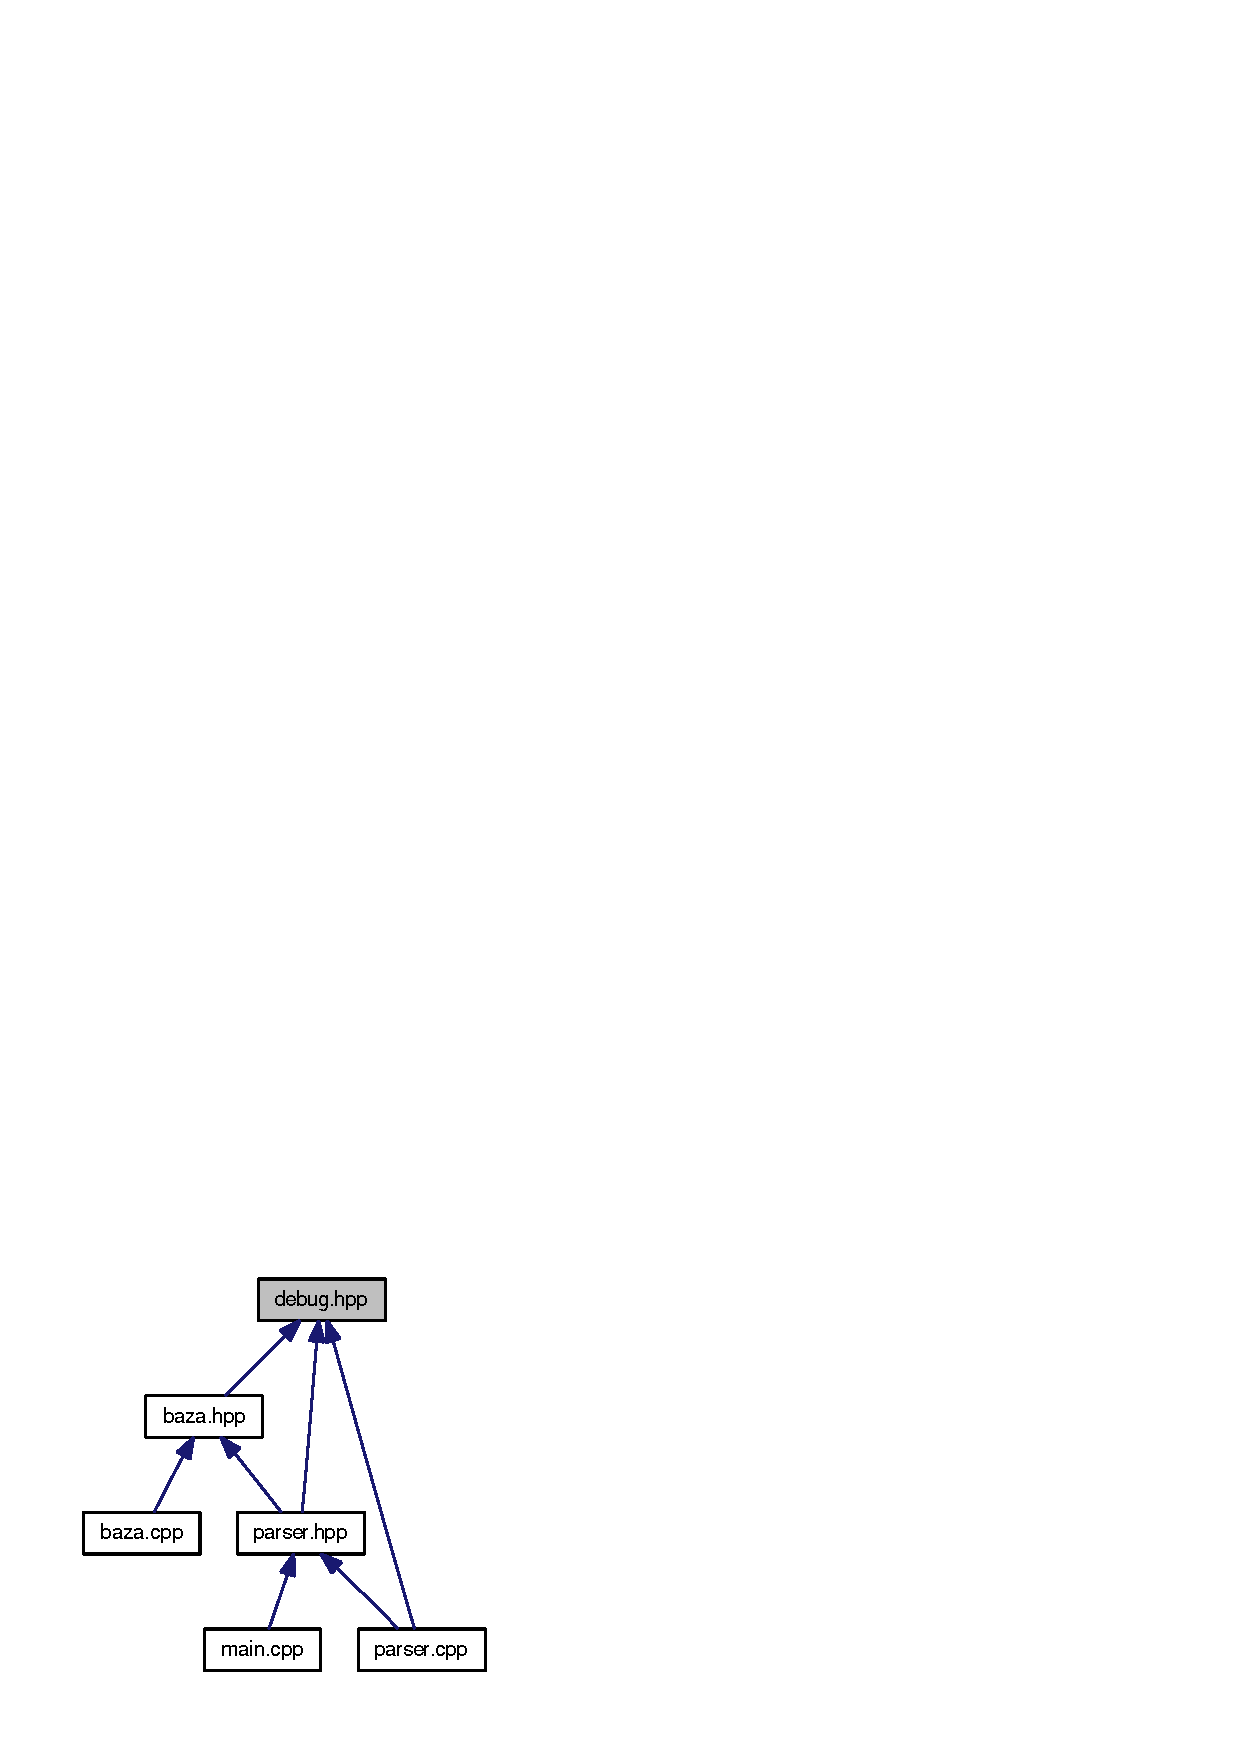
\includegraphics[width=118pt]{d8/d41/a00038}
\end{center}
\end{figure}
\subsection*{Definicje}
\begin{CompactItemize}
\item 
\#define \hyperlink{a00008_590af51ecfed28223c4e6ce02994241a}{info}(arg)
\item 
\#define \hyperlink{a00008_21ad5938437ed6d1865dd14c8d1871bc}{deb}(arg, arg2)
\item 
\#define \hyperlink{a00008_5bdec07ba0f5f220bcb40d5258725d95}{line}
\item 
\#define \hyperlink{a00008_9944134306515208e366f3f347ef3653}{Eline}
\item 
\#define \hyperlink{a00008_68b6fd999967bd748d50fc2014bc5903}{Eline2}(arg1, arg2)~;
\item 
\#define \hyperlink{a00008_51633d6d15647d74f756bcf969fc70ae}{info2}(arg, arg2)
\end{CompactItemize}


\subsection{Dokumentacja definicji}
\hypertarget{a00008_21ad5938437ed6d1865dd14c8d1871bc}{
\index{debug.hpp@{debug.hpp}!deb@{deb}}
\index{deb@{deb}!debug.hpp@{debug.hpp}}
\subsubsection[{deb}]{\setlength{\rightskip}{0pt plus 5cm}\#define deb(arg, \/  arg2)}}
\label{d4/dee/a00008_21ad5938437ed6d1865dd14c8d1871bc}




Definicja w linii 15 pliku debug.hpp.\hypertarget{a00008_9944134306515208e366f3f347ef3653}{
\index{debug.hpp@{debug.hpp}!Eline@{Eline}}
\index{Eline@{Eline}!debug.hpp@{debug.hpp}}
\subsubsection[{Eline}]{\setlength{\rightskip}{0pt plus 5cm}\#define Eline}}
\label{d4/dee/a00008_9944134306515208e366f3f347ef3653}




Definicja w linii 17 pliku debug.hpp.\hypertarget{a00008_68b6fd999967bd748d50fc2014bc5903}{
\index{debug.hpp@{debug.hpp}!Eline2@{Eline2}}
\index{Eline2@{Eline2}!debug.hpp@{debug.hpp}}
\subsubsection[{Eline2}]{\setlength{\rightskip}{0pt plus 5cm}\#define Eline2(arg1, \/  arg2)~;}}
\label{d4/dee/a00008_68b6fd999967bd748d50fc2014bc5903}




Definicja w linii 18 pliku debug.hpp.\hypertarget{a00008_590af51ecfed28223c4e6ce02994241a}{
\index{debug.hpp@{debug.hpp}!info@{info}}
\index{info@{info}!debug.hpp@{debug.hpp}}
\subsubsection[{info}]{\setlength{\rightskip}{0pt plus 5cm}\#define info(arg)}}
\label{d4/dee/a00008_590af51ecfed28223c4e6ce02994241a}




Definicja w linii 14 pliku debug.hpp.\hypertarget{a00008_51633d6d15647d74f756bcf969fc70ae}{
\index{debug.hpp@{debug.hpp}!info2@{info2}}
\index{info2@{info2}!debug.hpp@{debug.hpp}}
\subsubsection[{info2}]{\setlength{\rightskip}{0pt plus 5cm}\#define info2(arg, \/  arg2)}}
\label{d4/dee/a00008_51633d6d15647d74f756bcf969fc70ae}




Definicja w linii 19 pliku debug.hpp.\hypertarget{a00008_5bdec07ba0f5f220bcb40d5258725d95}{
\index{debug.hpp@{debug.hpp}!line@{line}}
\index{line@{line}!debug.hpp@{debug.hpp}}
\subsubsection[{line}]{\setlength{\rightskip}{0pt plus 5cm}\#define line}}
\label{d4/dee/a00008_5bdec07ba0f5f220bcb40d5258725d95}




Definicja w linii 16 pliku debug.hpp.